%!TEX root = ../dokumentation.tex

\chapter{Projektzeitplan}

Der Zeitplan wurde in \textit{Microsoft Project} erstellt. Die Dokumentation
unterscheidet zwei Ebenen. Der High-Level-Zeitplan stellt die Hauptphasen als
Gantt-Chart dar. Die Detailplanung bricht die Phasen in Arbeitspakete,
Abhängigkeiten und Ressourcen für die operative Steuerung herunter. Die
Planung orientiert sich am \ac{MOV}, die Lernplattform soll innerhalb von
zwölf Monaten eingeführt, getestet, pilotiert und konzernweit ausgerollt werden.
Zielprojektdauer \textbf{230 Arbeitstage}.

\section{Planungsgrundlage und Struktur des Zeitplans}

Der Projektzeitplan gliedert das Vorhaben in folgende Hauptphasen:

\begin{enumerate}
    \item Projektdefinition
    \item Detailplanung \& Architekturdesign
    \item Systemkonfiguration \& Integration
    \item Test \& Qualitätssicherung
    \item Pilotbetrieb
    \item Konzernweiter Rollout
    \item Stabilisierung \& Projektabschluss
\end{enumerate}

Die Phasen wurden in Teilpakete und konkrete Aktivitäten zerlegt und bilden so
die Grundlage für Terminsteuerung, Fortschrittskontrolle und Risikoüberwachung.
Der High-Level-Plan dient der Managementsicht, die operative Steuerung erfolgt
auf Basis der Detailplanung in \textit{Microsoft Project}.

\section{High-Level-Gantt-Chart}

Abbildung~\ref{fig:gantt-highlevel} zeigt den Projektzeitplan auf
Hauptphasenebene (Export aus \textit{Microsoft Project}).

\clearpage
\begin{landscape}
  \begin{figure}[htbp]
    \centering
    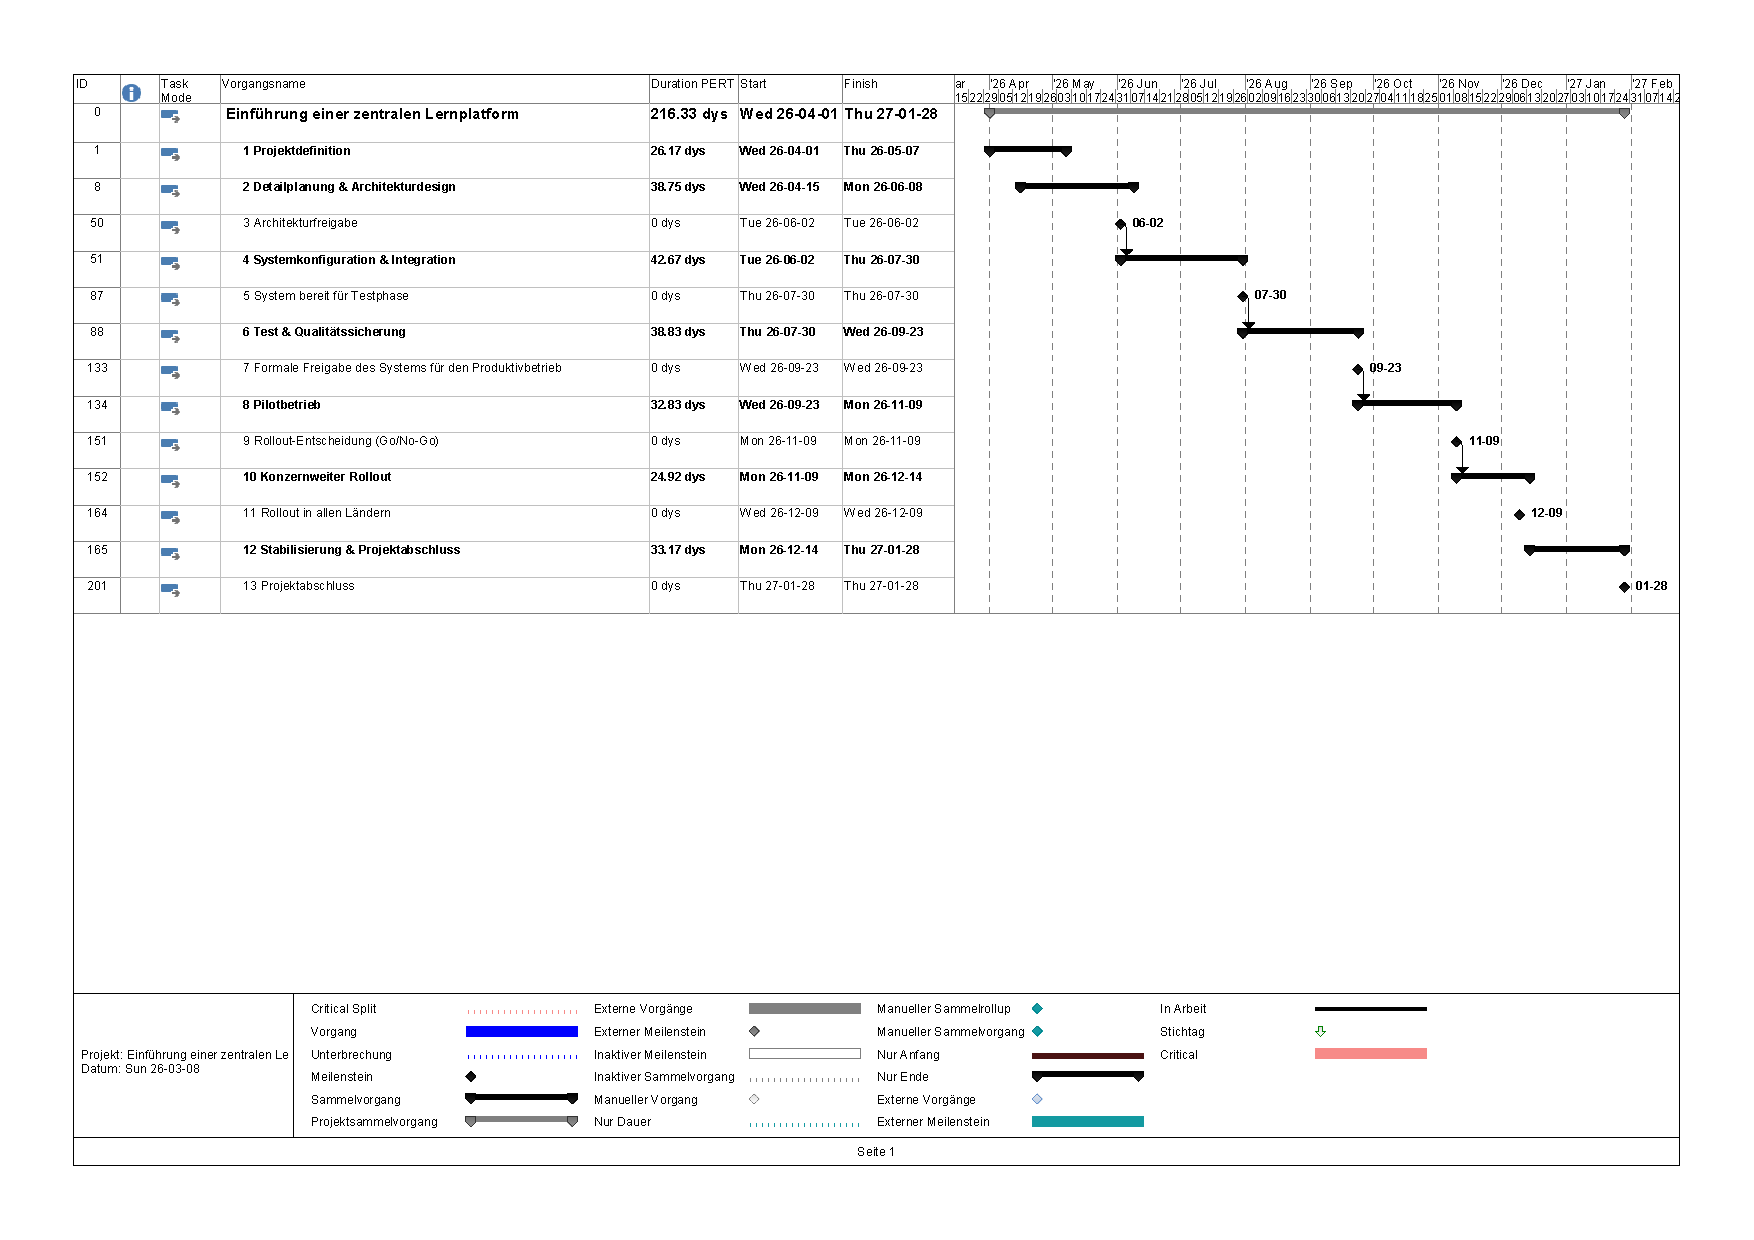
\includegraphics[width=\linewidth,height=\textheight,keepaspectratio,page=1]{images/pm26_gantt_1level_landscape.pdf}
    \caption{High-Level-Gantt-Chart des Projekts Lernplattform}
    \label{fig:gantt-highlevel}
  \end{figure}
\end{landscape}
\clearpage

\section{Meilensteine}

Zentrale Meilensteine bilden Abschluss- und Entscheidungszeitpunkte und
strukturieren das Projekt entlang der Hauptphasen.

\begin{xltabular}{\textwidth}{@{}>{\hsize=0.5\hsize}Xc>{\hsize=1.5\hsize}X@{}}
    \caption{Zentrale Meilensteine des Projekts} \label{tab:meilensteine} \\
    \toprule
    \textbf{Meilenstein} & \textbf{Datum} & \textbf{Bedeutung} \\
    \midrule
    \endfirsthead

    \toprule
    \textbf{Meilenstein} & \textbf{Datum} & \textbf{Bedeutung} \\
    \midrule
    \endhead

    \bottomrule
    \endfoot

    Projektstart                                          & 15.04.2026     & Formeller Start des Projekts nach Abschluss der initialen Projektdefinition und des Stakeholder Alignments.                   \\
    Architekturdesign abgeschlossen                       & 02.06.2026     & Abschluss der inhaltlichen Architekturarbeiten inklusive Zielarchitektur, Infrastruktur-, Integrations- und Reportingkonzept. \\
    Architekturfreigabe                                   & 02.06.2026     & Formelle Freigabe der Architektur als Voraussetzung für die nachgelagerte Systemkonfiguration und Integration.                \\
    Systemintegration abgeschlossen                       & 30.07.2026     & Abschluss der technischen Implementierung, Systemkonfiguration, Integrationen, Datenmigration und Reporting-Implementierung.  \\
    System bereit für Testphase                           & 30.07.2026     & Übergang aus der Implementierungsphase in die strukturierte Test- und Qualitätssicherung.                                     \\
    Formale Freigabe des Systems für den Produktivbetrieb & 23.09.2026     & Ergebnis der Test- und Abnahmephase, System für Pilotierung und produktiven Einsatz freigegeben.                      \\
    Rollout-Entscheidung (Go/No-Go)                       & 09.11.2026     & Entscheidungspunkt nach Pilotbetrieb und Readiness-Check für den konzernweiten Rollout.                                       \\
    Rollout in allen Ländern                              & 09.12.2026     & Abschluss des konzernweiten Rollouts und erfolgreiche Aktivierung der Ländergruppen.                                          \\
    Projektabschluss                                      & 28.01.2027     & Formeller Abschluss des Projekts nach Stabilisierung, Dokumentation, Übergabe und Abschlussbericht.                           \\
\end{xltabular}

\section{Probabilistische Terminbetrachtung mit \ac{PERT}}

Wegen Unsicherheiten bei mehreren Arbeitspaketen wurde die Terminplanung
ergänzend probabilistisch mit \ac{PERT} (\textit{Program Evaluation and Review
Technique}) vorgenommen. Pro Vorgang liegen drei Schätzungen vor (O optimistisch,
M wahrscheinlich, P pessimistisch).

Die erwartete Vorgangsdauer ergibt sich nach \ac{PERT} aus:

\begin{equation}
    E(T) = \frac{O + 4M + P}{6}
\end{equation}

Die Varianz ergibt sich zu

\begin{equation}
    Var(T) = \left(\frac{P - O}{6}\right)^2
\end{equation}

Auf Basis der \ac{PERT}-Auswertung für den kritischen Pfad ergeben sich für das
Projekt die in Tabelle~\ref{tab:pert-auswertung} dargestellten Kennzahlen.

\begin{xltabular}{\textwidth}{@{}lc@{}}
    \caption{Ergebnisse der \ac{PERT}-Analyse} \label{tab:pert-auswertung} \\
    \toprule
    \textbf{Kennzahl} & \textbf{Wert} \\
    \midrule
    \endfirsthead

    \toprule
    \textbf{Kennzahl} & \textbf{Wert} \\
    \midrule
    \endhead

    \bottomrule
    \endfoot

    Anzahl kritischer Vorgänge                               & 82               \\
    Gesamterwartungswert der Projektdauer                    & 223{,}00 Tage    \\
    Gesamtvarianz                                            & 41{,}72 Tage$^2$ \\
    Projektstandardabweichung                                & 6{,}46 Tage      \\
    Zieldauer                                                & 230{,}00 Tage    \\
    Z-Wert                                                   & 1{,}0837         \\
    Eintrittswahrscheinlichkeit für Einhaltung der Zieldauer & 86{,}0\,\%       \\
\end{xltabular}

Die erwartete Projektdauer liegt bei \textbf{223 Tagen}, bei Zieldauer
\textbf{230 Arbeitstagen} ergibt sich eine \textbf{Wahrscheinlichkeit von
86\,\%} zur Einhaltung. Der Zeitplan ist ambitioniert, aber realistisch. Die
Standardabweichung von 6{,}46 Tagen zeigt verbleibende Terminunsicherheiten,
wie bei einem Transformationsprojekt dieser Größe (Architektur, Integration,
Tests, Pilotierung, Rollout) erwartbar. Die \ac{PERT}-Betrachtung ergänzt den
Basisplan um eine realistischere Einschätzung der Terminrobustheit.

\section{Critical Path}

Der kritische Pfad umfasst Vorgänge, deren Verzögerung den Projektendtermin
verschiebt, und wird im Projektcontrolling besonders überwacht.

\clearpage
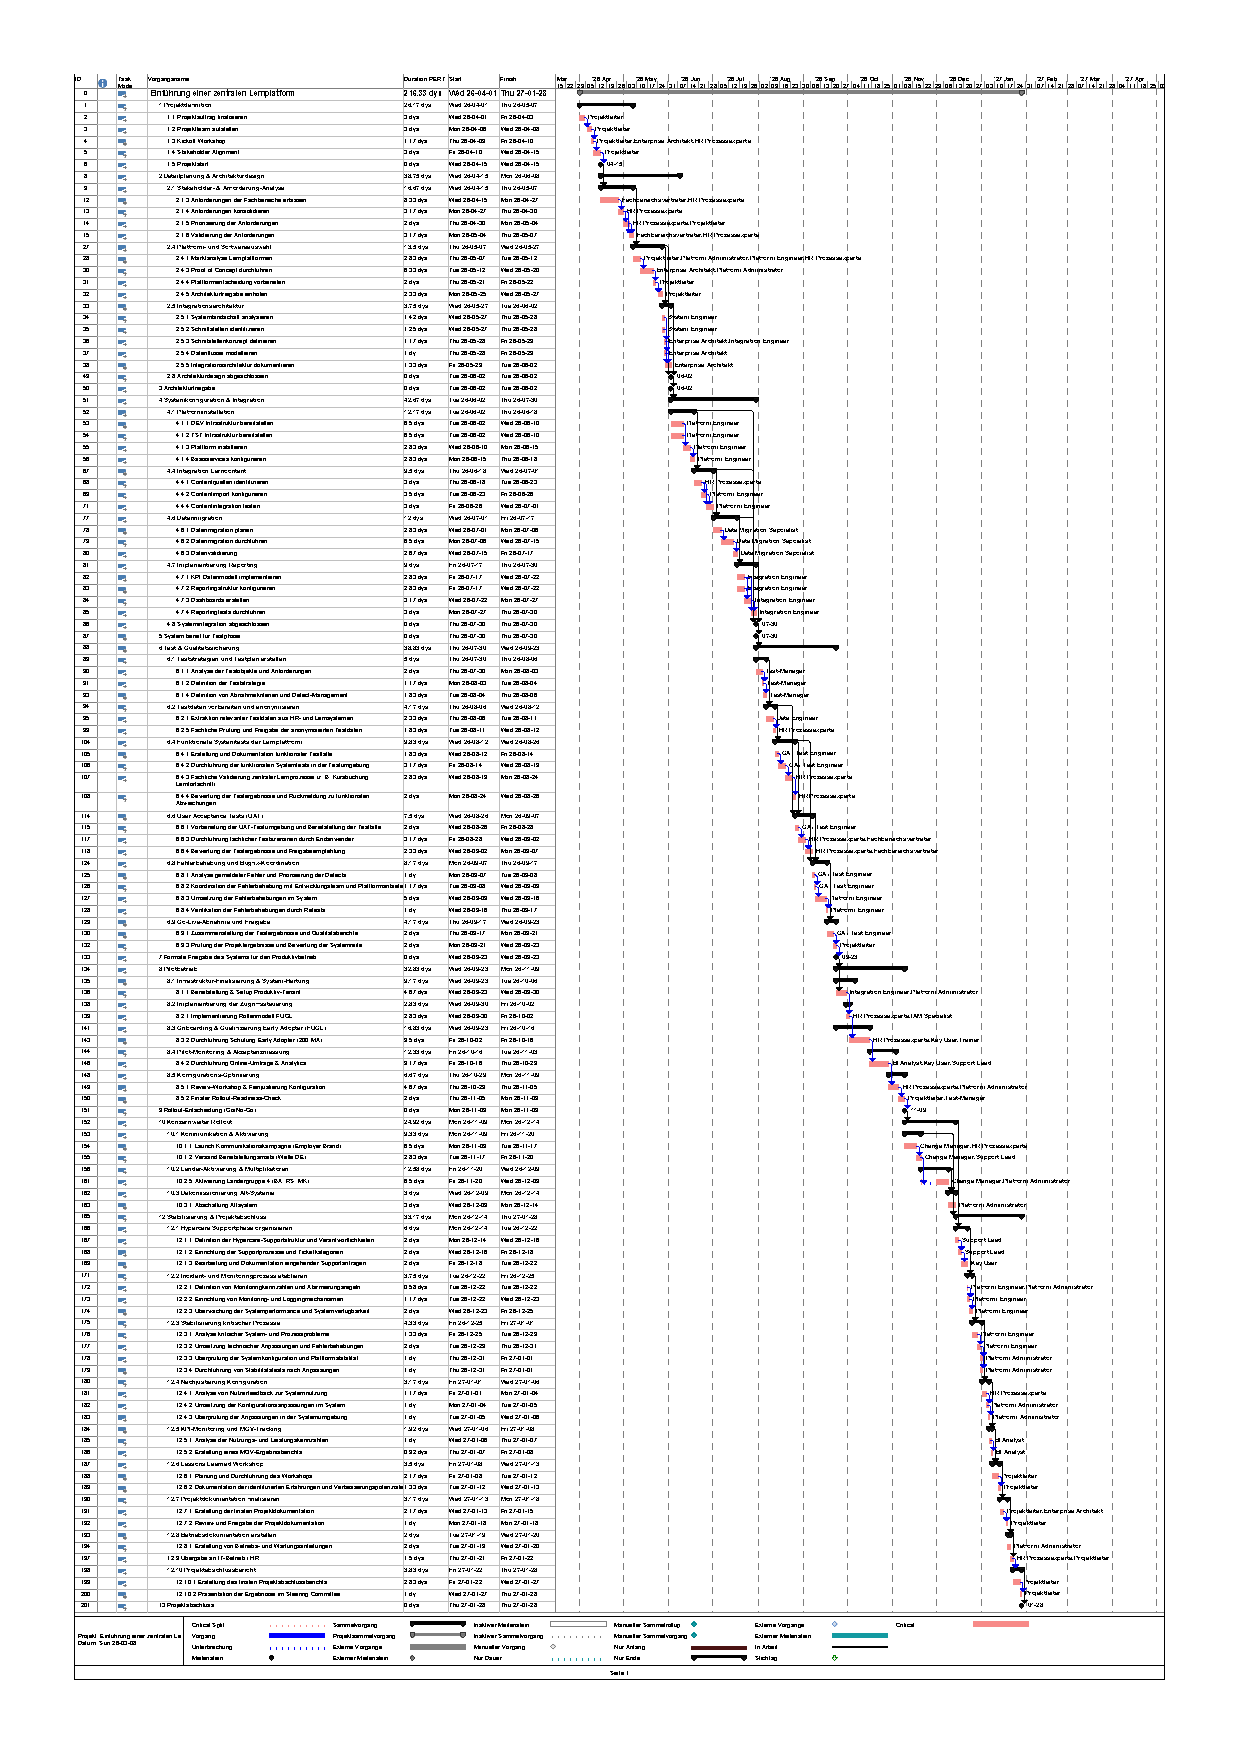
\includepdf[pages=1, fitpaper, pagecommand={%
    \thispagestyle{plain}%
    \refstepcounter{figure}%
    \addcontentsline{lof}{figure}{\protect\numberline{\thefigure}{Darstellung des kritischen Pfads}}%
    \label{fig:critical-path}%
}]{images/pm26_critical.pdf}
\clearpage

\section{Zusammenfassende Bewertung}

Der Projektzeitplan bildet das Vorhaben auf strategischer und operativer Ebene
ab. Der High-Level-Plan schafft Transparenz, die Feinplanung in
\textit{Microsoft Project} bildet die Grundlage für die operative Steuerung.
Die \ac{PERT}-Analyse berücksichtigt Unsicherheiten der Dauerplanung. Mit
223 Tagen erwarteter Dauer und 86\,\% Einhaltungswahrscheinlichkeit der
Zieldauer von 230 Tagen ist der Terminplan plausibel und geeignet für
Terminüberwachung und Projektcontrolling.